\documentclass{beamer}
\title{EMQX File Transfer Response Duplication}
\author{Ilya Averyanov}
\institute{EMQX}
\date{2023}
\usetheme{emqx}
\usepackage{listings}
\usepackage{color}
\usepackage{graphicx}
\usepackage{xcolor}
\usepackage{hyperref}
\definecolor{href}{rgb}{0,0,0.9375}
\hypersetup{
    pdfborderstyle={/S/U/W 1}, % underline links instead of boxes
    colorlinks=true,
    urlcolor=href
}
\lstset{frame=tb,
  aboveskip=3mm,
  belowskip=3mm,
  showstringspaces=false,
  columns=flexible,
  basicstyle={\small\ttfamily},
  numbers=none,
  numberstyle=\tiny\color{gray},
  keywordstyle=\color{blue},
  commentstyle=\color{dkgreen},
  stringstyle=\color{mauve},
  breaklines=true,
  breakatwhitespace=false,
  tabsize=2
}


\begin{document}

\frame{\titlepage}

\begin{frame}
    \frametitle{Response Duplication}
    \framesubtitle{Why Needed?}

    \begin{itemize}
        \item Not suitable for all cases, like MQTT bridging
        \item Not all client libraries have or have good support for QoS 1 PUBACKs
    \end{itemize}
\end{frame}


\begin{frame}
    \frametitle{Response Duplication}
    \framesubtitle{Simple Case}

    \begin{center}
        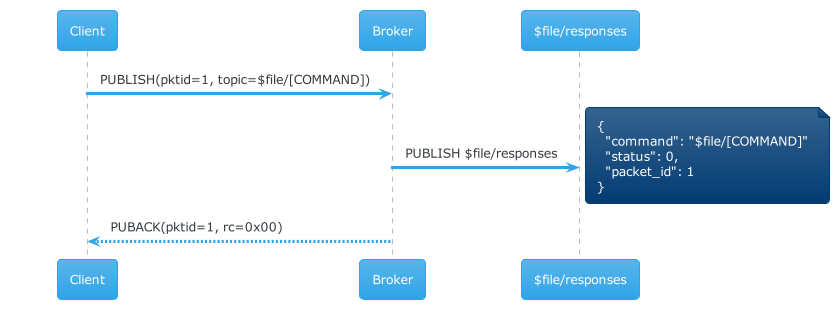
\includegraphics[width=10cm, keepaspectratio]{images/flow-topic-dup-simple.png}
    \end{center}
\end{frame}

\begin{frame}
    \frametitle{Response Duplication}
    \framesubtitle{Async Case, Variant 1}

    \begin{center}
        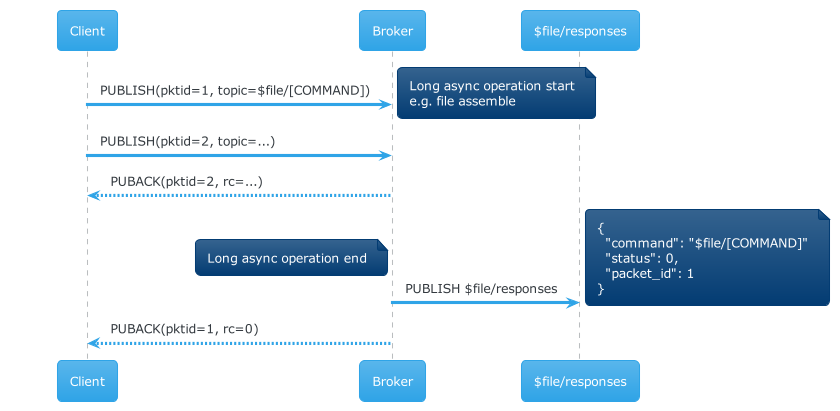
\includegraphics[width=10cm, keepaspectratio]{images/flow-topic-dup-async-1.png}
    \end{center}
\end{frame}

\begin{frame}
    \frametitle{Response Duplication}
    \framesubtitle{Async Case, Variant 2}

    \begin{center}
        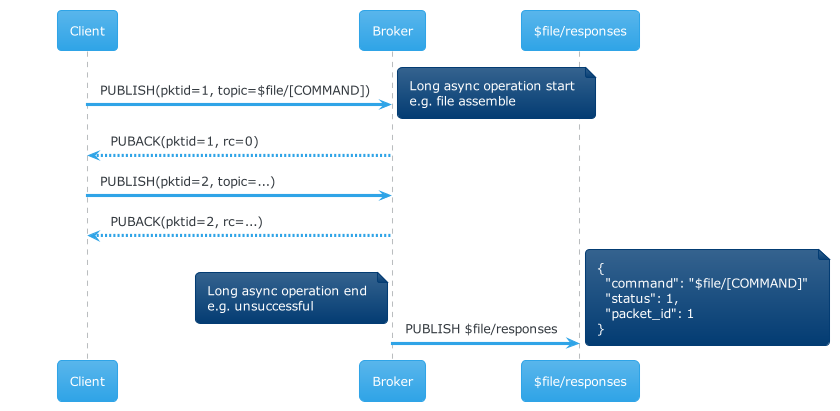
\includegraphics[width=10cm, keepaspectratio]{images/flow-topic-dup-async-2.png}
    \end{center}
\end{frame}

\begin{frame}
    \frametitle{Response Duplication}
    \framesubtitle{Multiple Async Case, Variant 1}

    \begin{center}
        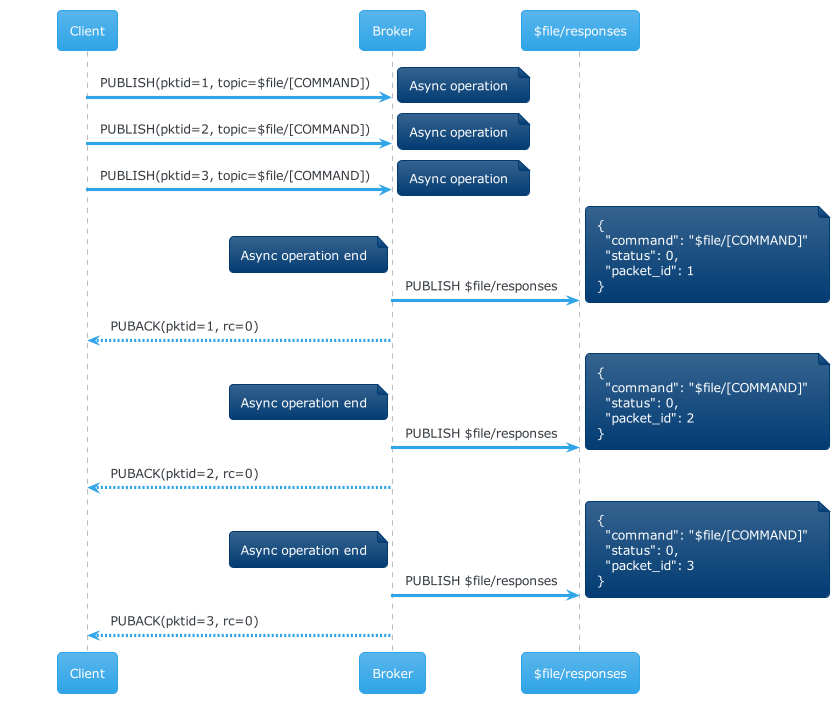
\includegraphics[width=8cm, keepaspectratio]{images/flow-topic-dup-async-multi-1.png}
    \end{center}
\end{frame}

\begin{frame}
    \frametitle{Response Duplication}
    \framesubtitle{Multiple Async Case, Variant 2}

    \begin{center}
        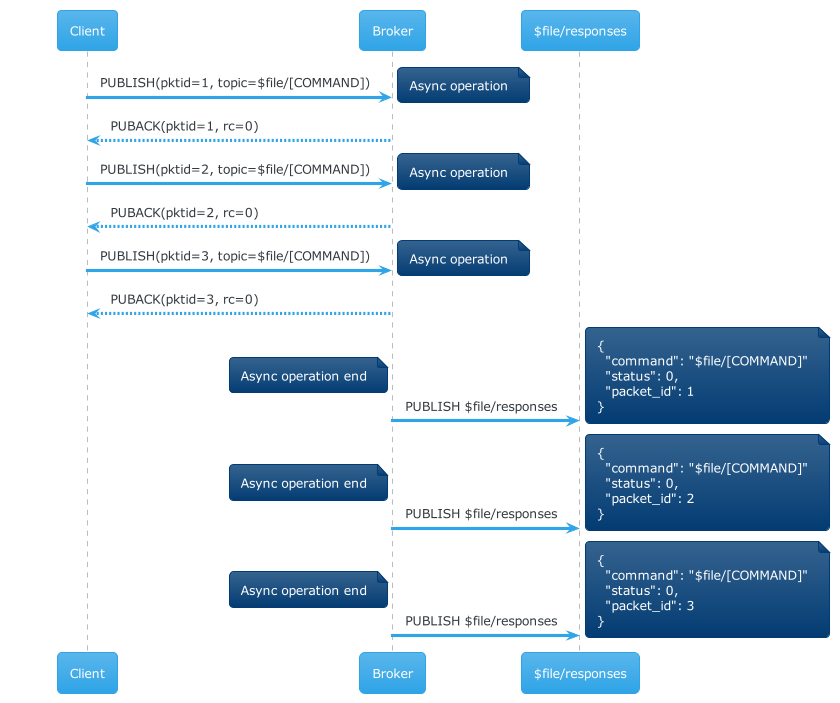
\includegraphics[width=8cm, keepaspectratio]{images/flow-topic-dup-async-multi-2.png}
    \end{center}
\end{frame}

\begin{frame}
    \frametitle{Response Duplication: Q}
    \framesubtitle{Flow Options}
    Which flow options should we support?
    \begin{itemize}
        \item Async PUBACK (implemented)
        \item Async PUBACK + PUBLISH to Topic
        \item Sync PUBACK ($rc = 0$) + PUBLISH to Topic
    \end{itemize}
\end{frame}

\begin{frame}
    \frametitle{Response Duplication}
    \framesubtitle{Async PUBACK}
    \begin{itemize}
        \item \lstinline{The Variable Header component of many of the MQTT Control Packet types
        includes a Two Byte Integer Packet Identifier field}
        \item For \href{https://emqx.atlassian.net/l/cp/YDANuEv9}{"AWS-friendly" FT} we may have thousands of async PUBLISHes
        \item We have only 65536 packet identifiers
    \end{itemize}
\end{frame}

\begin{frame}
    \frametitle{Response Duplication: Q}
    \framesubtitle{Default topic scheme for responses}
    \begin{itemize}
        \item \lstinline{$file/[FILEID]/response}
        \item \lstinline{$file/response}
        \item Other variant?
    \end{itemize}
    For custom topics, we support REQUEST/RESPONSE topic scheme. Should we support custom
    default response topic scheme in config?
\end{frame}

\begin{frame}
    \begin{center}
        Thank you!
    \end{center}
\end{frame}

\end{document}
